%%%%%%%%%%%%%%%%%%%%%%%%%%%%%%%%%%%%%%%%%%%%%%%%%%%%%%%%%%%%%%%%%%%%%%%%%%%%%
% Rich Meier 3/15/14 - Final Project - UCT Monte Carlo Othello Project %%%%%%%%%%%%%%%%%%%%%%%%%%%%%%%%%%%%%%%%%%%%%%%%%%%%%%%%%%%%%%%%%%%%%%%%%%%%%%
% Header
\documentclass[12pt,letterpaper]{article}
\usepackage[utf8]{inputenc}
\usepackage{amsmath}
\usepackage{amsfonts}
\usepackage{amssymb}
\usepackage{graphicx}
\usepackage[margin=1in]{geometry}
%\usepackage{booktabs}
%\usepackage{colortbl}
%%%%%%%%%%%%%%%%%%%%%%%%%%%%%%%%%%%%%%%%%%%%%%%%%%%%%%%%%%%%%%%%%%%%%%%%%%%%%%
%\definecolor{grey}{RGB}{190,190,190}
% Begin
\begin{document}

\title{\vspace{-1in}Final Project -- CS 533 \\ Monte Carlo UCT Algorithm Applied to Playing Othello}
\author{Rich Meier}
\date{\today}
\maketitle

\vspace{-.5in}
\section{Introduction}
The following report will cover the development of a Monte-Carlo-based Othello player. The algorithm described below will use the UCT algorithm to play Othello against multiple opponents in a adversarial environment. We have developed the UCT Monte-Carlo-based tree search algorithm in python, and created it to be compatible with a pre-designed Othello game environment. The hope is that our algorithm will succeed in beating the provided AI 'minimax lookahead algorithm'.

Section~\ref{back} will provide some fundamental background knowledge on the game Othello, as well as the theoretical components of the UCT tree algorithm.  Next, Section~\ref{meth} will cover the methodology and important coding used to validate and evaluate our algorithm. Section~\ref{results} will discuss the results of the experimentation described in the previous section, and finally Section~\ref{conc} will conclude.

\section{Background Information}
\label{back}

The following discusses the fundamental components of playing Othello, as well as implementing the UCT algorithm.

\subsection{Playing Othello}

The game of Othello is actually quite simple. It is a two player game where each player seeks to maximize the number of chips on the board that are their own color (black or white). The board is typically an eight by eight square, and play continues on the board while either player still has a legal move or until the board is full. Legal moves must have at least one adjacent token that is the opponent's color, and the current player's own color is either diagonally, vertically, or horizontally aligned with the move.  

In order to maximize the number of captured pieces on the board, there are a few widely accepted strategic positions.  Specifically, capturing corner squares is considered best because they are impossible for the opposing player to recapture. Side squares are also advantageous because the eliminate capturing capability in the orthogonal direction. Figure~\ref{fig1} depicts a typical Othello game about midway through competition.

\begin{figure}[!h]
\begin{center}
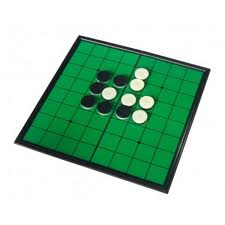
\includegraphics[scale=1]{othello_board}
\caption{\textit{The Othello game -- a mid-game snapshot.}}
\label{fig1}
\end{center}
\end{figure}

\subsection{UCT Algorithm}
The UCT algorithm is a Monte-Carlo tree based algorithm that utilizes explore/exploit tactics to build a decision tree at each independent action level. Simply put, whenever the agent must make a decision, the UCT algorithm rolls-out multitudes of independent trajectories that utilize the best policy according to the tree. If the trajectory reaches a point that the tree has not yet simulated, a default policy is executed in order to simply estimate values for that particular sub-tree.  This in turn adds and updates a new leaf node as well as the nodes along the path of the trajectory - starting at the root node.

The values that are learned via this algorithm are approximate Q-values.  This means that node has a value that is specifically related to both the state of the game at that point, as well as ``best" action that the agent can take at that point. More formally, the UCT algorithm will return a value that is a summation of the best known Q-value and an exploring value.  This is represented by the policy relationship in Equation~\ref{eq1} below:
\begin{equation}
\label{eq1}
\Pi_{uct}(s) = MAX_a \left( Q(s,a) + c*\sqrt{\frac{\log(n(s))}{n(s,a)}} \right)
\end{equation}

\section{Methodology}
\label{meth}

\subsection{Othello Python Code}

The project consists of a 3rd-party Othello environment. Some small changes were made to the code in order to implement UCT and use it as an agent in the Othello environment.

The 3rd-party environment is centered around `othello.py', which contains the class `game'. This class maintains the Othello board, describes whose turn it is, enumerates the moves that are available, and allows moves to be played. It also keeps score. Our only change to this was to add a score function that is independent of player turn (positive for the black pieces, negative for the white pieces). The file `game2.py' provides the `player' class, which is initialized with a policy function (that takes a position and returns a move). Game2.py also provides a play() function which takes a game state and two players and simulates the rest of the game. We modified play() to return the final score of the game, since it is helpful to know who wins after simulating games. 

This the entire simulator environment. However, there are two more files that were included with this package: `othello\_gui.py', which provides a simple GUI for a human to play against any opponent player, and `minimax.py', which implements an agent that uses minimax alpha-beta search with a variable lookahead depth and a custom evaluation function. This minimax agent, was implemented using a more traditional AI method, and it was a useful benchmark for us in evaluating the performance of our agent.

\subsection{Custom Code}

Our code consists of two files. CS533\_Final.py is the file that runs simulations and was used for experiments. It also contains some simple policies, one random policy that chooses from the available moves, and one greedy policy that chooses the move that will capture the greatest number of the opponent's pieces. These simple policies were the two available default policies for our simulations (playing against themselves) in UCT.

UCT\_tree.py is the file that contains the bulk of the UCT algorithm. Overall it is almost independent of the game of Othello, relying only on generic functions of the simulator such as the game class' generate\_moves() and play\_move() functions, as well as access to a simulator that returns the overall reward. The class Tree consists of a list of nodes, as well as some parameters of the UCT algorithm: the time budget per move, the value c of the tree policy, and the policy function to be used when simulating results.

Each node corresponds to a certain state (and contains a game object). Nodes keep track of their children (by indices of the children in the tree's list of nodes), the number of times each action was taken, and the rewards received from simulations following those actions. Nodes can also calculate the value of their actions according to the UCT tree policy (when given a value for c) as well as the estimated reward from each action.

The tree class builds a tree of nodes over many simulated trajectories and relies upon them to decide the best action. This begins in the policy() function, which runs trajectories from the root node until the time allotted runs out, and then picks the move with the highest Q-value.

The trajectory() function is the most involved, and does most of the tree building. At a given node, trajectory() will first check if all of the nodes' actions have been taken at least once. If some have not, it randomly chooses one, takes that action, adds a new node to the tree, and simulates the game from that new node based on the default policy (random or greedy). If all actions have been taken, trajectory() uses the tree policy and its explore-exploit nature to choose an action to take, and recursively calls trajectory on the node resulting from that action, which will eventually lead to the base case, where trajectory is called on a node with some actions that have not yet been simulated. In the base case, the resulting reward from the simulation is returned and used to update the action counts and action rewards on each node, and this is propagated up the tree as the recursion unwinds.

Our implementation incidentally relies on the fact that Othello is deterministic, so once an action leads to a child node (that is, a game state), it will always lead there. For a nondeterministic simulation, this would need to be replaced by a mapping from game states to value indices. Otherwise our entire implementation could be reused on a simulator of an entirely unrelated game.

Finally, our evaluation in CS533\_Final.py consists of nested loops over several sets of parameters, including the default policy, opponent players, values of c, time budgets per-move, and the number of games to play at each configuration. This makes it easy to collect results for any number of possible configurations. However, especially with larger time budgets, the runtime becomes prohibitive, and thus we used this setup to select interesting values, to cut down on the number of final configurations tested.

\subsection{Policies}

\subsection{Experimentation}



\begin{enumerate}
\item Default simulation policy outside of the tree policy (greedy and random)
\item C-values for exploration within tree.
\item Different Opponents (random, greedy, minimax-3, minimax-4, minimax-5)
\item Play first or play second.
\item 10 games each average scores.

\end{enumerate}

\section{Results}
\label{results}


\section{Conclusion}
\label{conc}





\end{document}
